\subsection{Example \#5: generate and analyze synthetic data }
\label{S:EXAMPLESYNTHETICDATA}


\subsubsection{Purpose}
This example illustrates how to create a synthetic time series using OpenBDLM.
The objective is to create a 4-years long time series with an acceleration stationary baseline, and a yearly periodic pattern as well as a autoregressive process superimposed into it. 
The timestep is 1 day.
This example corresponds to the OpenBDLM demo presented in Section~\ref{S:OPENBDLMGETTINGSTARTED}.

\begin{figure*}[h!]
\centering
\begin{subfigure}{\linewidth}
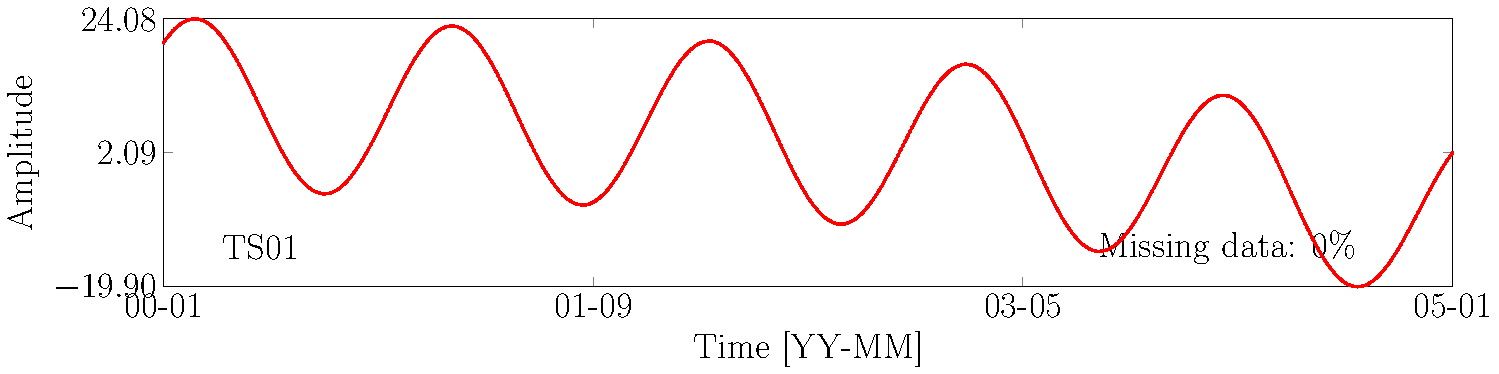
\includegraphics[width=0.9\linewidth]{./docfigs/Example_SYNTHETIC/raw/ALL_AMPLITUDES.pdf} 
\caption{Amplitude}
\end{subfigure}
\begin{subfigure}{\linewidth}
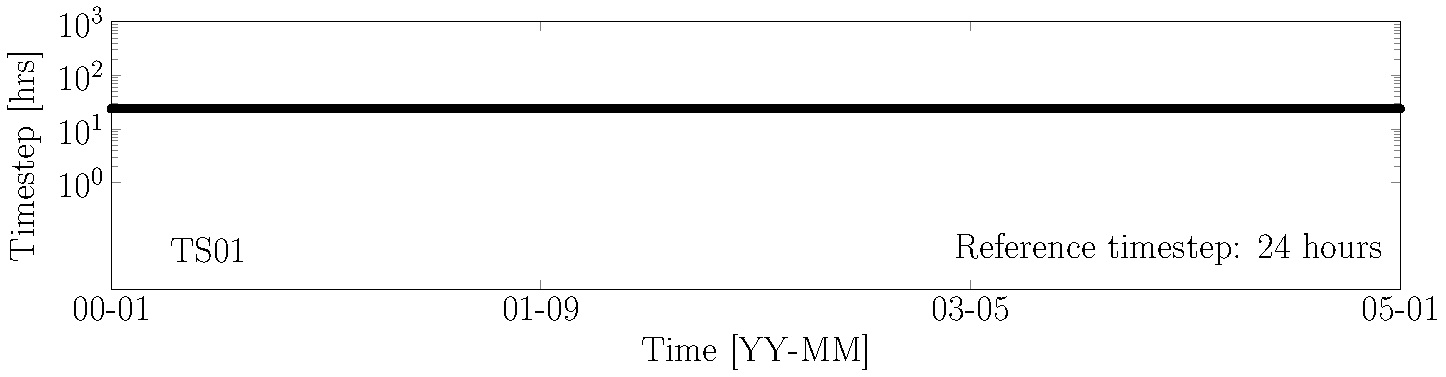
\includegraphics[width=0.9\linewidth]{./docfigs/Example_SYNTHETIC/raw/ALL_TIMESTEPS.pdf}
\caption{Timestep}
\end{subfigure}
\begin{subfigure}{\linewidth}
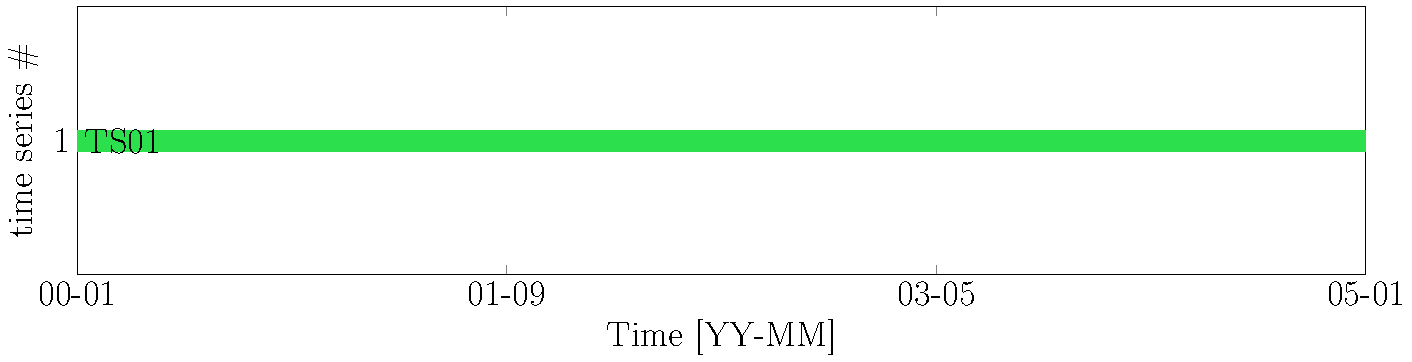
\includegraphics[width=0.9\linewidth]{./docfigs/Example_SYNTHETIC/raw/AVAILABILITY.pdf}
\caption{Availability}
\end{subfigure}
\caption{Data used in example \#5}.
\label{fig:DataSummaryRawSynthetic}
\end{figure*}


\subsubsection{Model description}
The model includes one model class, and the block components are 
\begin{gather*}
\textbf{x}=[x^{\mathtt{L}}, x^{\mathtt{T}}, x^{\mathtt{LA}}, x^{\mathtt{P1}\text{,yearly}}, x^{\mathtt{P2}\text{,yearly}}, x^{\mathtt{AR}}].
\end{gather*}
The associated model parameters are
\begin{gather*}
\bm\theta=\{\sigma_{w}^{\mathtt{LA}}, p^{\mathtt{PD}, \text{yearly}}, \sigma_{w}^{\mathtt{PD}, \text{yearly}}, \phi^{\mathtt{AR}}, \sigma_{w}^{\mathtt{AR}}, \sigma_{v,\text{D}}\} 
 \end{gather*}
The model parameters values assigned by default from OpenBDLM are
\begin{gather*}
\bm\theta^{\text{defaut}}=[ 1\times10^{-8}, 365.24, 0, 0.75, 0.01, 0.01].
\end{gather*}
The default initial hidden states mean and covariance values, and model probability are 
\begin{align*}
\bm \mu^{\text{defaut}}_{0} & = [	 10  , -1\times10^{-5}  ,	-0.001	,	10  ,  	10    ,	0  ]^{\intercal}, \text{and} \\
\bm\Sigma^{\text{defaut}}_{0} & = \text{diag}[ 0.01  ,	0.01  ,	0.01  	,0.04  ,	0.04  ,	0.01 ], \\
 \pi_{0}^{1,\text{default}} & = 1.
 \end{align*}
The synthetic data generated from this model structure, model parameters values and initial hidden states values are presented in Figure~\ref{fig:DataSummaryRawSynthetic}.
The hidden states computed using the same (i.e. true) model structure, model parameters values and initial hidden states values are presented in Figure~\ref{fig:SYNTHETICOptimizedOptimized}.

\subsubsection{Run the example from command line interaction}

This section explains how to run the example \#4, that is, how to generate the synthetic data presented in Figure~\ref{fig:DataSummaryRawSynthetic}, and estimate the hidden states as presented in Figure~\ref{fig:SYNTHETICOptimizedOptimized}.


\begin{enumerate}
\item Start OpenBDLM. Type \colorbox{light-gray}{\lstinline[basicstyle = \mlttfamily \small, backgroundcolor = \color{light-gray}]!OpenBDLM_main;!}.
\item Choose the interactive tool. Type \colorbox{light-gray}{\lstinline[basicstyle = \mlttfamily \small, backgroundcolor = \color{light-gray}]!0!}.
\item Enter the project name. Type \colorbox{light-gray}{\lstinline[basicstyle = \mlttfamily \small, backgroundcolor = \color{light-gray}]!Example_SYNTHETIC!}. 
\item Generate synthetic data. Type \colorbox{light-gray}{\lstinline[basicstyle = \mlttfamily \small, backgroundcolor = \color{light-gray}]!yes!}. 
\item Provide the number of time series. Type \colorbox{light-gray}{\lstinline[basicstyle = \mlttfamily \small, backgroundcolor = \color{light-gray}]!1!}.
\item Provide  the date corresponding of the first data sample. Type \colorbox{light-gray}{\lstinline[basicstyle = \mlttfamily \small, backgroundcolor = \color{light-gray}]!2000-01-01!}.
\item Provide  the date corresponding of the last data sample. Type \colorbox{light-gray}{\lstinline[basicstyle = \mlttfamily \small, backgroundcolor = \color{light-gray}]!2005-01-01!}.
\item Provide  the timestep in day. Type \colorbox{light-gray}{\lstinline[basicstyle = \mlttfamily \small, backgroundcolor = \color{light-gray}]!1!}.
\item Select the number of model classes. Type \colorbox{light-gray}{\lstinline[basicstyle = \mlttfamily \small, backgroundcolor = \color{light-gray}]!1!}. 
\item Select the model block components. Type \colorbox{light-gray}{\lstinline[basicstyle = \mlttfamily \small, backgroundcolor = \color{light-gray}]![13 31 41]!}. The Figure~\ref{fig:DataSummaryRawSynthetic} should popup on screen.
\item Access hidden states estimation menu. Type \colorbox{light-gray}{\lstinline[basicstyle = \mlttfamily \small, backgroundcolor = \color{light-gray}]!3!}. 
\item Estimate the filtered hidden states. Type \colorbox{light-gray}{\lstinline[basicstyle = \mlttfamily \small, backgroundcolor = \color{light-gray}]!1!}. The estimation should be similar to the results presented in Figure~\ref{fig:SYNTHETICOptimizedOptimized}.
\item Save and quit OpenBDLM. Type \colorbox{light-gray}{\lstinline[basicstyle = \mlttfamily \small, backgroundcolor = \color{light-gray}]!Q!}.
\end{enumerate}



%First, choose the interactive tool by typing \colorbox{light-gray}{\lstinline[basicstyle = \mlttfamily \small, backgroundcolor = \color{light-gray}]!0!}.
%Secondly, provide a project name (i.e. \lstinline[basicstyle = \mlttfamily \small, backgroundcolor = \color{light-gray}]!Example_SYNTHETIC!).
%Then, answer \colorbox{light-gray}{\lstinline[basicstyle = \mlttfamily \small, backgroundcolor = \color{light-gray}]!yes!} to indicate that you would like to create synthetic data.
%Finally, type \colorbox{light-gray}{\lstinline[basicstyle = \mlttfamily \small, backgroundcolor = \color{light-gray}]!1!} to create one single synthetic time series. 
%
%\subsection{Step 2: define the time step vector}
%
%Type \colorbox{light-gray}{\lstinline[basicstyle = \mlttfamily \small, backgroundcolor = \color{light-gray}]!2000-01-01!}, \colorbox{light-gray}{\lstinline[basicstyle = \mlttfamily \small, backgroundcolor = \color{light-gray}]!2005-01-01!} and \colorbox{light-gray}{\lstinline[basicstyle = \mlttfamily \small, backgroundcolor = \color{light-gray}]!1!}, to provide the date corresponding of the first and last data sample of the synthetic data, as well as the timestep in days.


%\subsection{Step 3: configure the model}
%
%First, the program requests the number of model class.
%In this example, we would like to create synthetic data with no anomaly.
%In such case, we type \colorbox{light-gray}{\lstinline[basicstyle = \mlttfamily \small, backgroundcolor = \color{light-gray}]!1!} to choose a single model class.
%Then, OpenBDLM asks for the type of block component.
%As mentionned earlier, the objective is to create synthetic time series data with an acceleration stationary baseline, and a yearly periodic pattern superimposed into it. 
%%The presence of a daily periodic pattern is unclear.
%Therefore, we choose \colorbox{light-gray}{\lstinline[basicstyle = \mlttfamily \small, backgroundcolor = \color{light-gray}]![13 31 41]!}.
%This model considers a trend stationary model with a yearly periodic pattern, and an autoregressive process to be more realistic.
%At this time, three figures  that represent the amplitude, timestep and availability of the newly created synthetic data (as shown in Figure~\ref{fig:DataSummaryRawSynthetic}) should popup on the screen.
%Type \colorbox{light-gray}{\lstinline[basicstyle = \mlttfamily \small, backgroundcolor = \color{light-gray}]!Q!} to save and quit.
%
%\subsection{Step 4: explore the model}
%From the main menu, type  \colorbox{light-gray}{\lstinline[basicstyle = \mlttfamily \small, backgroundcolor = \color{light-gray}]!11!} to see what are the values of model parameters which have been assigned to create the synthetic data.
%The model totalizes 6 model parameters, that is 
%\begin{gather*}
%\bm\theta=\{\sigma_{w, \text{D}}^{LA}, p^{\text{PD1}}_{\text{D}}, \sigma_{w,\text{D}}^{\text{PD1}}, \phi^{AR}_{\text{D}}, \sigma_{w,\text{D}}^{AR}, \sigma_{v,\text{D}}\} 
% \end{gather*}
%The default model parameters values are 
%\begin{gather*}
%\bm\theta^{\text{default}}=\{1\times10^{-8}, 365.24, 0, 0.75, 0.01, 0.01\}, 
%\end{gather*}
%in agreement with the values indicated in Table~\ref{table:defaultsynthetic}.
%Type \colorbox{light-gray}{\lstinline[basicstyle = \mlttfamily \small, backgroundcolor = \color{light-gray}]!R!} to return to the main menu.
%Then, type \colorbox{light-gray}{\lstinline[basicstyle = \mlttfamily \small, backgroundcolor = \color{light-gray}]!12!} the see that the default initial hidden states mean, covariance  and model probability values are 
%\begin{align*}
% \bm \mu^{1,\text{default}}_{0} & = [	10  , -1\times10^{-5}  ,	-0.001	,	10  ,  	10    ,	0         ]^{\intercal}, \text{and} \\
% \text{diag}(\bm\Sigma^{1,\text{default}}_{0})  & = [	0.01  ,	0.01  ,	0.01  	,0.04  ,	0.04  ,	0.01     ], \text{and} \\
% \pi_{0}^{1,\text{default}} & = 1.
%\end{align*}
%respectively, in agreement with the values indicated in Table~\ref{table:defaultsynthetic}.
%Type \colorbox{light-gray}{\lstinline[basicstyle = \mlttfamily \small, backgroundcolor = \color{light-gray}]!R!} to return to the main menu.

%\begin{figure*}[h!]
%\centering
%\begin{subfigure}{\linewidth}
%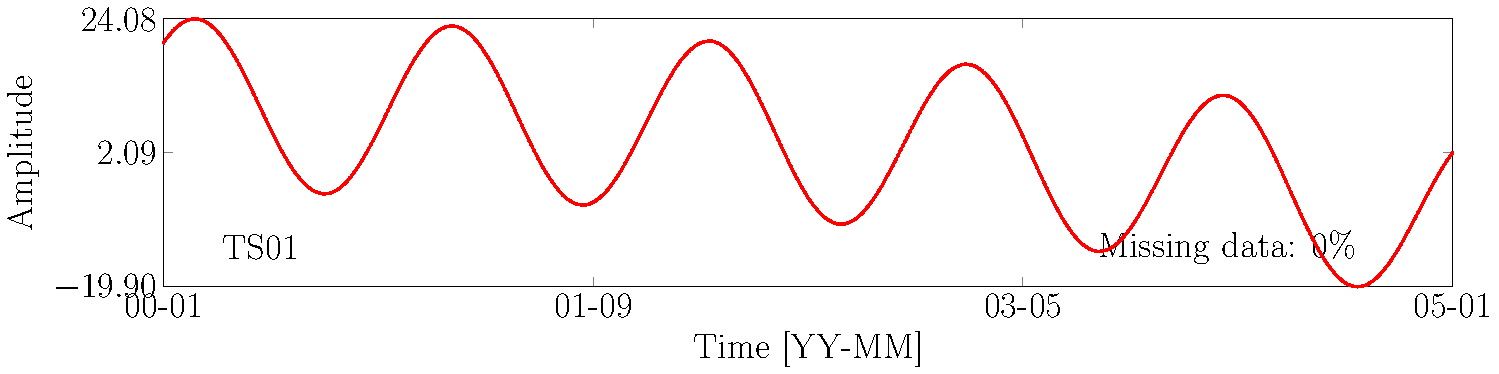
\includegraphics[width=0.9\linewidth]{./docfigs/Example_SYNTHETIC/raw/ALL_AMPLITUDES.pdf} 
%\caption{Amplitude}
%\end{subfigure}
%\begin{subfigure}{\linewidth}
%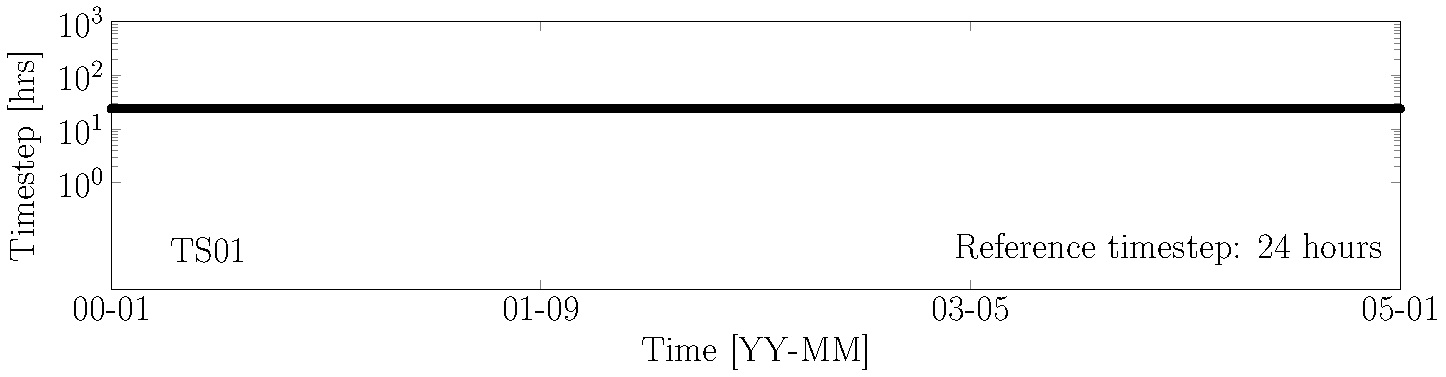
\includegraphics[width=0.9\linewidth]{./docfigs/Example_SYNTHETIC/raw/ALL_TIMESTEPS.pdf}
%\caption{Timestep}
%\end{subfigure}
%\begin{subfigure}{\linewidth}
%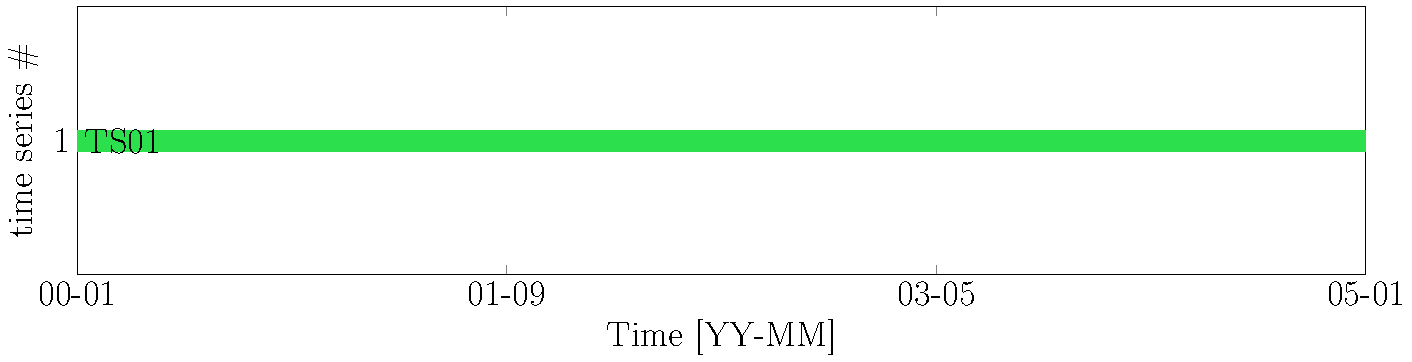
\includegraphics[width=0.9\linewidth]{./docfigs/Example_SYNTHETIC/raw/AVAILABILITY.pdf}
%\caption{Availability}
%\end{subfigure}
%\caption{Data used in example \#4}.
%\label{fig:DataSummaryRawSynthetic}
%\end{figure*}


%\subsection{Step 5: estimate the hidden states}
%
%From the main menu, type  \colorbox{light-gray}{\lstinline[basicstyle = \mlttfamily \small, backgroundcolor = \color{light-gray}]!3!}, then \colorbox{light-gray}{\lstinline[basicstyle = \mlttfamily \small, backgroundcolor = \color{light-gray}]!1!} to estimate the filtered hidden states using the default model parameters and default initial hidden states values.
%The value of the log-likelihood is $4976$, and the estimated hidden states are presented in Figure~\ref{fig:SYNTHETICDefaultDefaultExample4}.
%For each figure, the red dashed line represents the true known values of the hidden states.
%
%\begin{figure*}[h!]
%\centering
%\begin{subfigure}{\linewidth}
%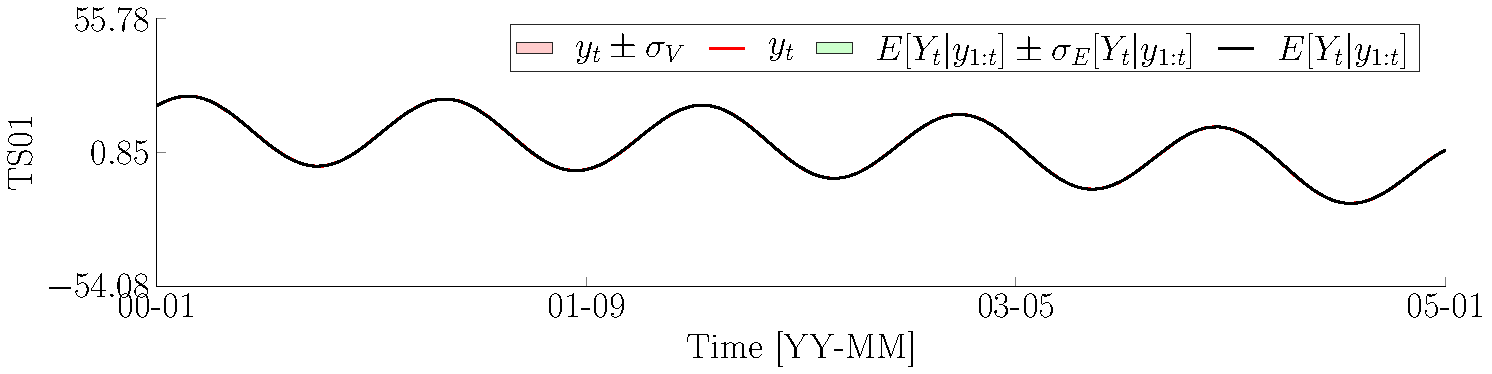
\includegraphics[width=0.9\linewidth]{./docfigs/Example_SYNTHETIC/default/TS01_ObservedPredicted.pdf}
%\caption{Observed and estimated displacement data}
%\end{subfigure}
%\begin{subfigure}{\linewidth}
%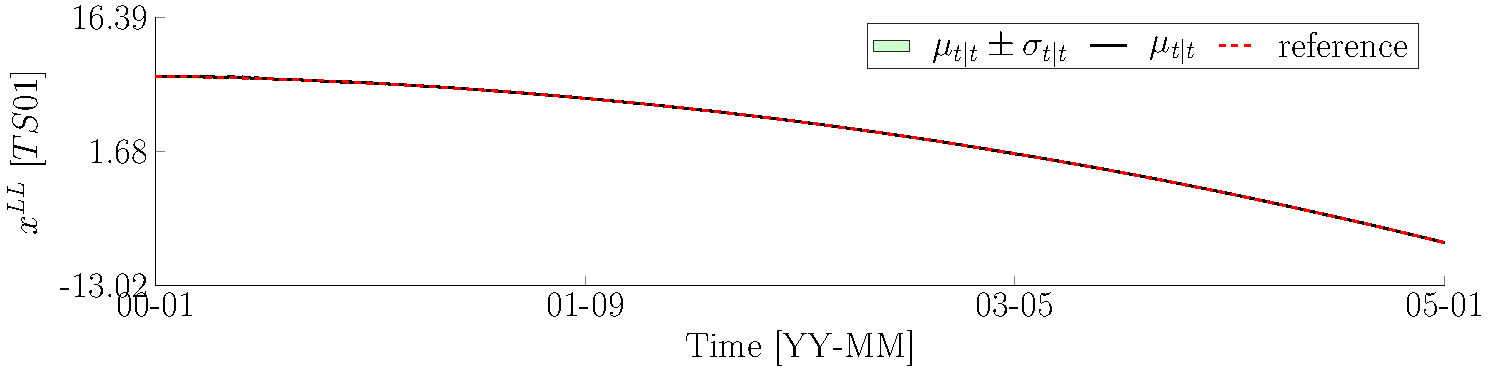
\includegraphics[width=0.9\linewidth]{./docfigs/Example_SYNTHETIC/default/TS01_LL_1.pdf} 
%\caption{Estimated displacement local level component}
%\end{subfigure}
%\begin{subfigure}{\linewidth}
%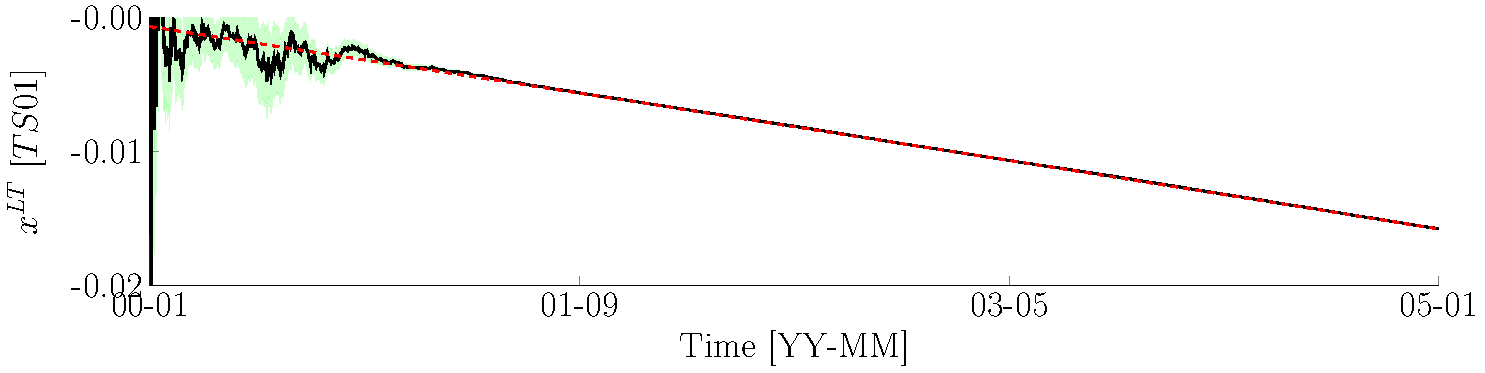
\includegraphics[width=0.9\linewidth]{./docfigs/Example_SYNTHETIC/default/TS01_LT_2.pdf}
%\caption{Estimated displacement local trend component.}
%\end{subfigure}
%\begin{subfigure}{\linewidth}
%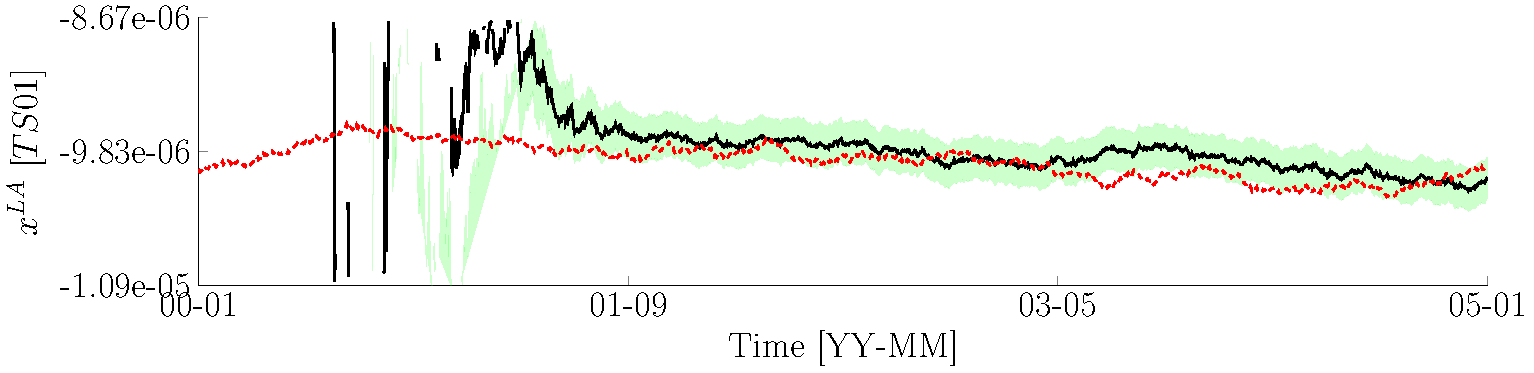
\includegraphics[width=0.9\linewidth]{./docfigs/Example_SYNTHETIC/default/TS01_LA_3.pdf}
%\caption{Estimated displacement local acceleration component.}
%\end{subfigure}
%\end{figure*}
%\begin{figure*}[h!]
%\ContinuedFloat
%\begin{subfigure}{\linewidth}
%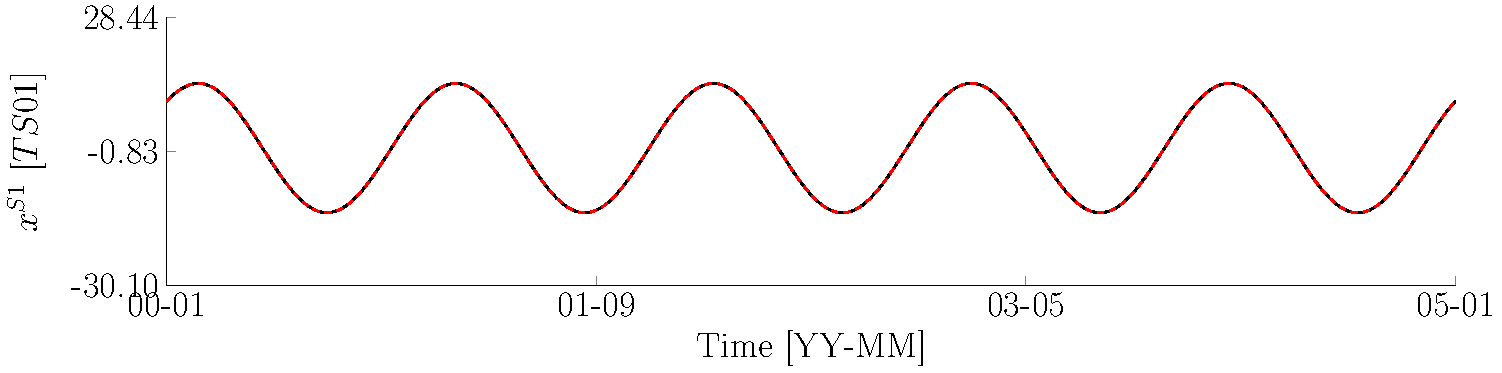
\includegraphics[width=0.9\linewidth]{./docfigs/Example_SYNTHETIC/default/TS01_S1_4.pdf}
%\caption{Estimated displacement yearly periodic component (first hidden state)}
%\end{subfigure}
%\begin{subfigure}{\linewidth}
%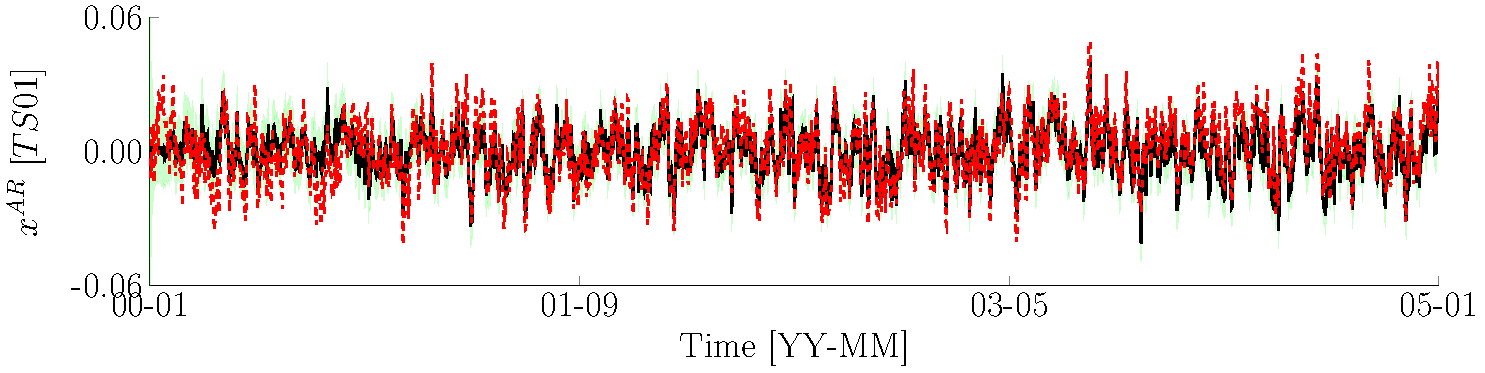
\includegraphics[width=0.9\linewidth]{./docfigs/Example_SYNTHETIC/default/TS01_AR_6.pdf} 
%\caption{Estimated displacement autoregressive component}
%\end{subfigure}
%\caption{Estimated results using OpenBDLM default model parameters and default initial hidden states. The hidden states are estimated from the data presented in Figure~\ref{fig:DataSummaryRawSynthetic}a. The solid line and shaded area represent the mean and standard deviation of the estimated hidden states, respectively. The red dashed line represent the true the hidden state value.}
%\label{fig:SYNTHETICDefaultDefaultExample4}
%\end{figure*}

%\subsection{Step 6: estimate the initial hidden states}
%
%From the main menu, type  \colorbox{light-gray}{\lstinline[basicstyle = \mlttfamily \small, backgroundcolor = \color{light-gray}]!2!}, to optimize the initial hidden states value.
%The estimated initial hidden states mean and covariance values are 
%\begin{align*}
%\bm \mu^{*}_{0} & = [	10 ,   	-0.00103,	-9.68\times10^{-6},	10   , 	10    ,	-0.0106  ]^{\intercal}, \text{and} \\
% \text{diag}(\bm\Sigma^{*}_{0}) & = [	2.35\times10^{-5}	, 1.33\times10^{-9},	3.3\times10^{-14}	, 1.9\times10^{-6}	, 2.03\times10^{-6}	,0.000353    ], 
% \end{align*}
% respectively.
%Once it is done, type  \colorbox{light-gray}{\lstinline[basicstyle = \mlttfamily \small, backgroundcolor = \color{light-gray}]!3!}, and then  \colorbox{light-gray}{\lstinline[basicstyle = \mlttfamily \small, backgroundcolor = \color{light-gray}]!1!} to compute the filtered hidden states using the optimized model parameters and optimized initial hidden states.
%The value of the log-likelihood is $5011$.
%The estimated hidden states are presented in Figure~\ref{fig:SYNTHETICOptimizedOptimized}.


\begin{figure*}[h!]
\centering
\begin{subfigure}{\linewidth}
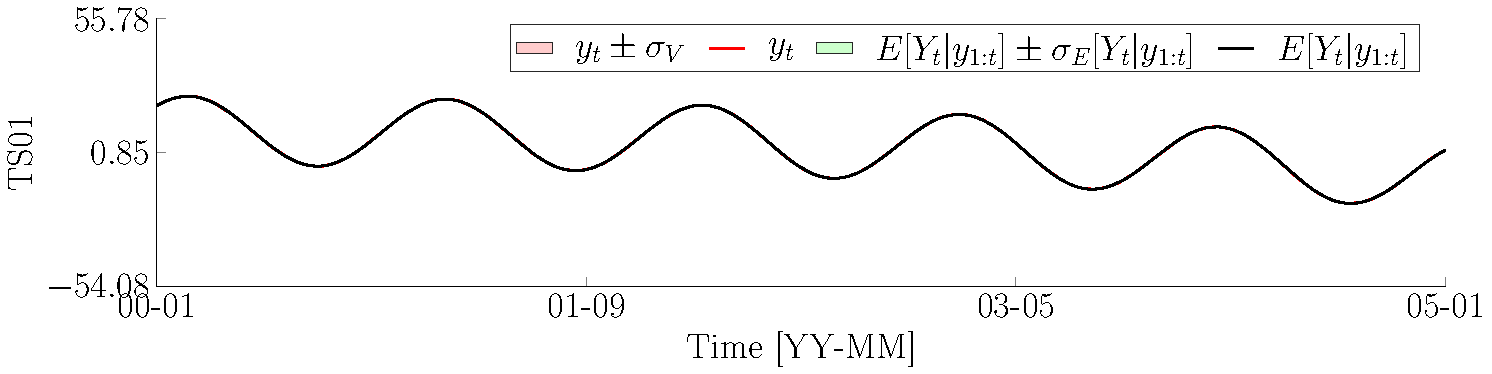
\includegraphics[width=0.9\linewidth]{./docfigs/Example_SYNTHETIC/optim_param_optim_initialhiddenstate/TS01_ObservedPredicted.pdf}
\caption{Observed and estimated displacement data}
\end{subfigure}
\begin{subfigure}{\linewidth}
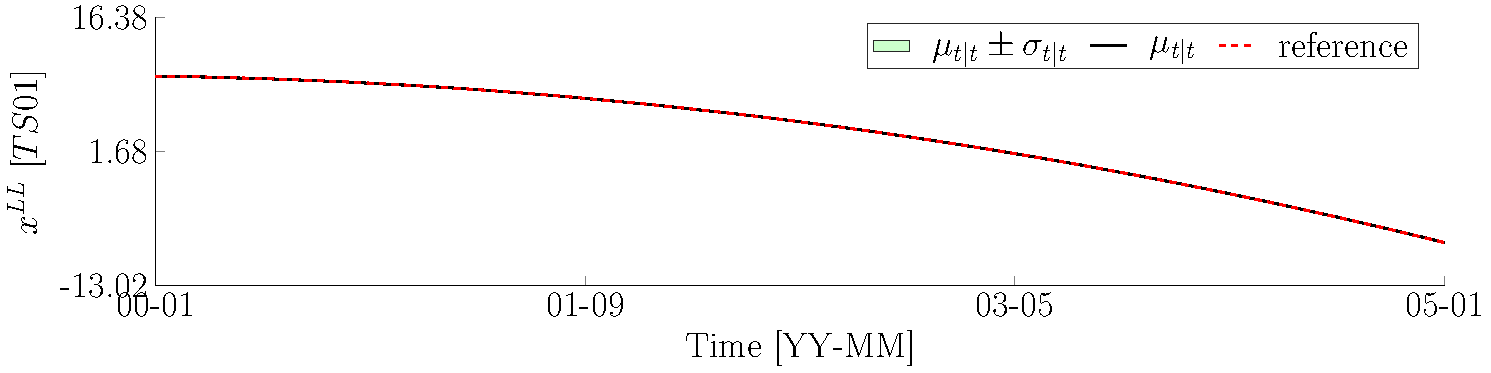
\includegraphics[width=0.9\linewidth]{./docfigs/Example_SYNTHETIC/optim_param_optim_initialhiddenstate/TS01_LL_1.pdf} 
\caption{Estimated displacement level component}
\end{subfigure}
\begin{subfigure}{\linewidth}
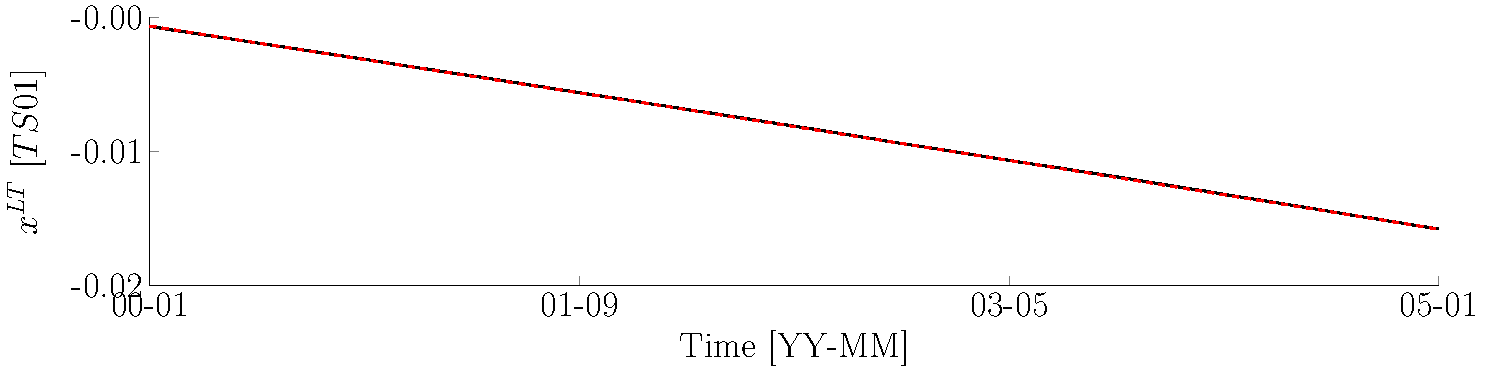
\includegraphics[width=0.9\linewidth]{./docfigs/Example_SYNTHETIC/optim_param_optim_initialhiddenstate/TS01_LT_2.pdf}
\caption{Estimated displacement trend component.}
\end{subfigure}
\begin{subfigure}{\linewidth}
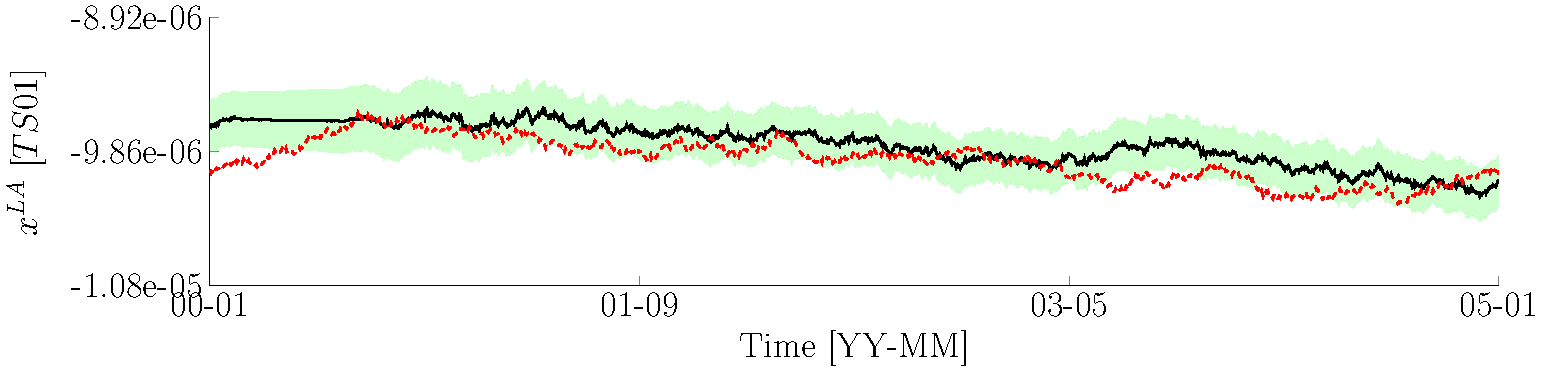
\includegraphics[width=0.9\linewidth]{./docfigs/Example_SYNTHETIC/optim_param_optim_initialhiddenstate/TS01_LA_3.pdf}
\caption{Estimated displacement local acceleration component.}
\end{subfigure}
\end{figure*}
\begin{figure*}[h!]
\ContinuedFloat
\begin{subfigure}{\linewidth}
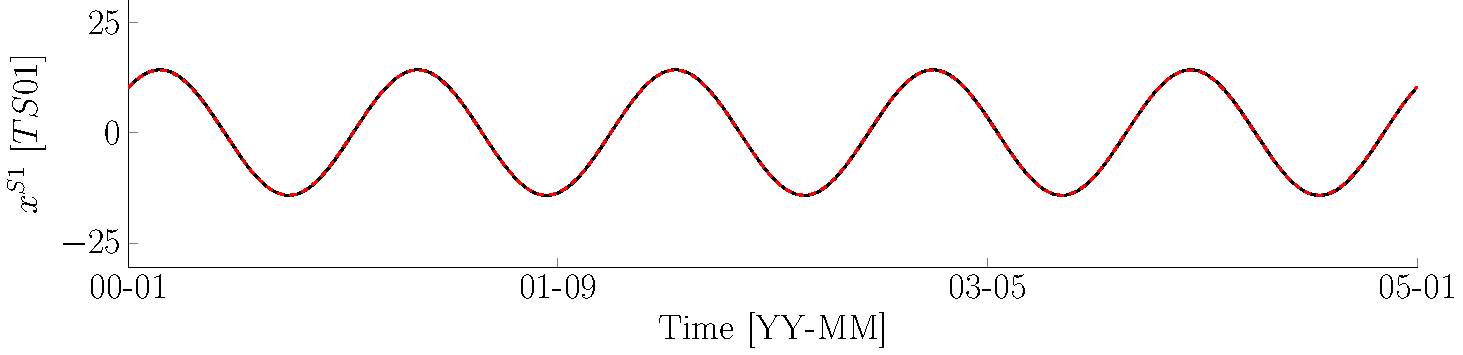
\includegraphics[width=0.9\linewidth]{./docfigs/Example_SYNTHETIC/optim_param_optim_initialhiddenstate/TS01_S1_4.pdf}
\caption{Estimated displacement yearly periodic component (first hidden state)}
\end{subfigure}
\begin{subfigure}{\linewidth}
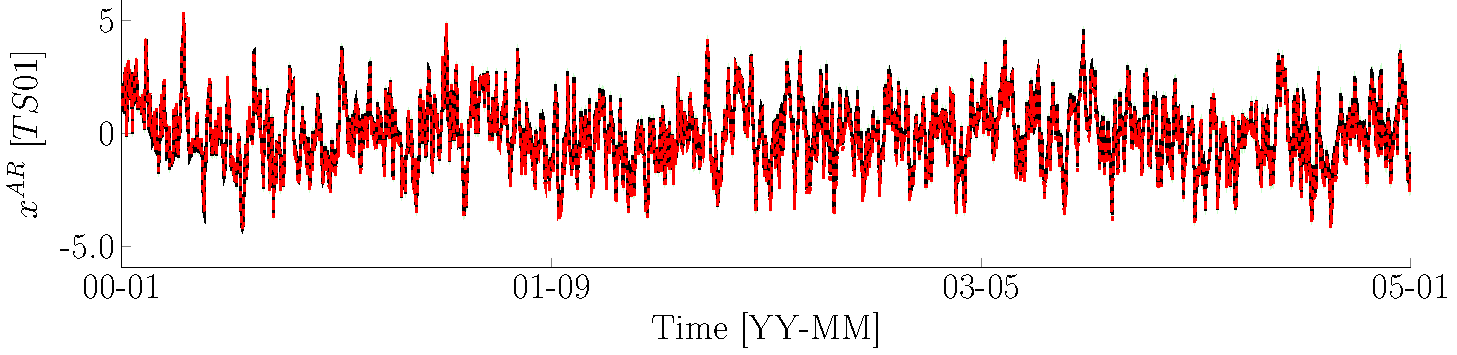
\includegraphics[width=0.9\linewidth]{./docfigs/Example_SYNTHETIC/optim_param_optim_initialhiddenstate/TS01_AR_6.pdf} 
\caption{Estimated displacement autoregressive component}
\end{subfigure}
\caption{Estimated results using OpenBDLM default model parameters and optimized initial hidden states. The hidden states are estimated from the data presented in Figure~\ref{fig:DataSummaryRawSynthetic}a. The solid line and shaded area represent the mean and standard deviation of the estimated hidden states, respectively. The red dashed line represent the true the hidden state value.}
\label{fig:SYNTHETICOptimizedOptimized}
\end{figure*}


